\newcommand{\note}[1]{{\footnotesize\textrm{#1}}}

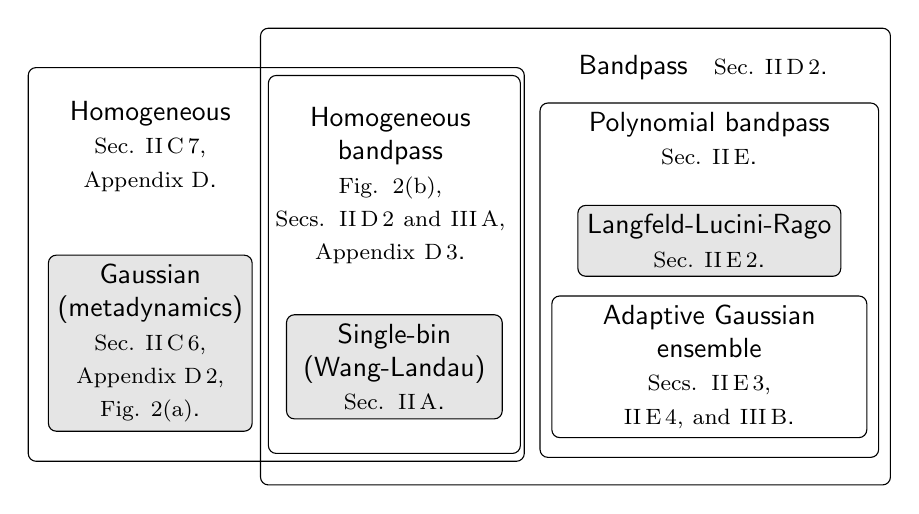
\begin{tikzpicture}[scale=1.0, every node/.style={rounded corners=0.1cm, align=center}]\sffamily
  \node[]
    (H) at (-1.6, 3.5)
    {Homogeneous\\
    \note{Sec. II\,C\,7,}\\
    \note{Appendix D}.
    };

  \node[draw, fill=white!90!black]
    (G) at (-1.6, 1.0)
    {Gaussian\\
    (metadynamics)\\
    \note{Sec. II\,C\,6,}\\
    \note{Appendix D\,2,}\\
    \note{Fig. 2(a)}.
    };

  \node[draw, minimum width=6.3cm, minimum height=5cm]
    (Hbox) at (0.0, 2) {};

  \node[draw, minimum width=8cm, minimum height=5.8cm]
    (Bbox) at (3.8, 2.1) {};

  \node[draw, minimum width=3.2cm, minimum height=4.8cm]
    (HBbox) at (1.5, 2) {};

  \node[draw, text width={width("Single-bin ABCD")}, fill=white!90!black]
    (sbin) at (1.5, 0.7)
    {Single-bin\\
    (Wang-Landau)\\
    \note{Sec. II\,A}.
    };

  \node[text width={width("Homogeneous AAAAAA")}]
    (HB) at (1.45, 3.0)
    {Homogeneous\\bandpass\\
    \note{Fig. 2(b),}\\
    \note{Secs. II\,D\,2 and III\,A,}\\
    \note{Appendix D\,3}.
    };

  \node[] (B) at (5.5, 4.5)
    {Bandpass \;
    \note{Sec. II\,D\,2}.
    };

  \node[draw, minimum width=4.3cm, minimum height=4.5cm]
    (PBbox) at (5.5, 1.8) {};

  \node[] (PB) at (5.5, 3.6)
    {Polynomial bandpass\\
    \note{Sec. II\,E}.
    };

  \node[draw, fill=white!90!black]
    (LLR) at (5.5, 2.3)
    {Langfeld-Lucini-Rago\\
    \note{Sec. II\,E\,2}.
    };

  \node[draw, text width={width("Adaptive Gaussian ABCD")}]
    (AGE) at (5.5, 0.7)
    {Adaptive Gaussian\\ensemble\\
    \note{Secs. II\,E\,3, II\,E\,4, and III\,B}.
    };

\end{tikzpicture}

